% 第 16 题(1)乙：浮力 F 随水平位移 x 的变化（pgfplots）
% 空间周期 0.4 m：x=0 与 0.4 处为最大值 F1，x=0.2 处为最小值 F2
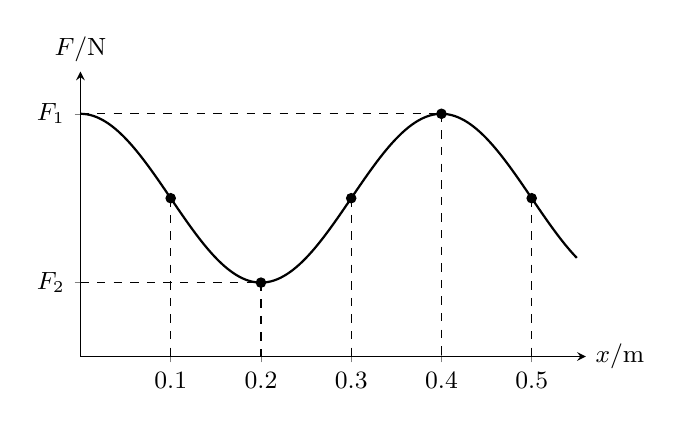
\begin{tikzpicture}
  \begin{axis}[
      width=8cm, height=5.2cm,
      axis lines=middle,
      xlabel={$x$/m}, ylabel={$F$/N},
      xmin=0, xmax=0.56, ymin=0, ymax=1.35,
      xtick={0.1,0.2,0.3,0.4,0.5},
      ytick={0.35,1.15}, yticklabels={$F_2$,$F_1$},
      xlabel style={anchor=west}, ylabel style={anchor=south},
      font=\small]
    \addplot[thick, domain=0:0.55, samples=160]
      {0.75+0.40*cos(deg(2*pi*x/0.4))};
    \addplot[only marks, mark=*, mark size=1.7pt] coordinates {
      (0.1,0.75) (0.2,0.35) (0.3,0.75) (0.4,1.15) (0.5,0.75)};
    \draw[dashed] (0,1.15) -- (0.4,1.15); \draw[dashed] (0.4,1.15) -- (0.4,0);
    \draw[dashed] (0,0.35) -- (0.2,0.35); \draw[dashed] (0.2,0.35) -- (0.2,0);
    \draw[dashed] (0.1,0.75) -- (0.1,0);
    \draw[dashed] (0.3,0.75) -- (0.3,0);
    \draw[dashed] (0.5,0.75) -- (0.5,0);
    \node[below left, font=\scriptsize] at (axis cs:0,0) {$O$};
  \end{axis}
\end{tikzpicture}
